\subsection{Sigmoid en ReLU}
In dit experiment bekijken we het verschil tussen de activatie functies, sigmoid en ReLU. Het verschil tussen de twee is dat sigmoid een bovengrens van 1 heeft, terwijl ReLU geen boven grens heeft.

\begin{table}[ht]
    \centering
      $\begin{array}{ c || l | c  | c | c}
   \text{Aantal verborgen knopen} & & \text{Sigmoid} & \text{ReLU} \\ \hline
     \multirow{2}{*}{4}  &    \text{Aantal correct}       & 23 & 30 \\ \cline{2-4}
     &   \text{Percentage \% correct} & 46 & 60 \\ \cline{2-4}
     &   \text{Tijd (in secondes)}   & 8.881 & 1.412 \\ \hline \hline 
     \multirow{2}{*}{16} &   \text{Aantal correct}       & 36 & 30 \\ \cline{2-4}
     &   \text{Percentage \% correct} & 72 & 60 \\ \cline{2-4}
     &   \text{Tijd (in secondes)} & 26.516 & 4.219\\ \hline \hline
      \multirow{2}{*}{24} &   \text{Aantal correct}       & 41 & 31\\ \cline{2-4}
     &   \text{Percentage \% correct} & 82 & 62\\ \cline{2-4}
     &   \text{Tijd (in secondes)}  & 38.275 & 6.166\\ \hline
      \end{array}$
    \caption{Aantal correcte antwoorden over 50 executies met activatie functies sigmoid en ReLU met verschillende aantallen verborgen knopen}
    \label{tab:relu}
\end{table}
\begin{figure}[ht!]
    \centering
    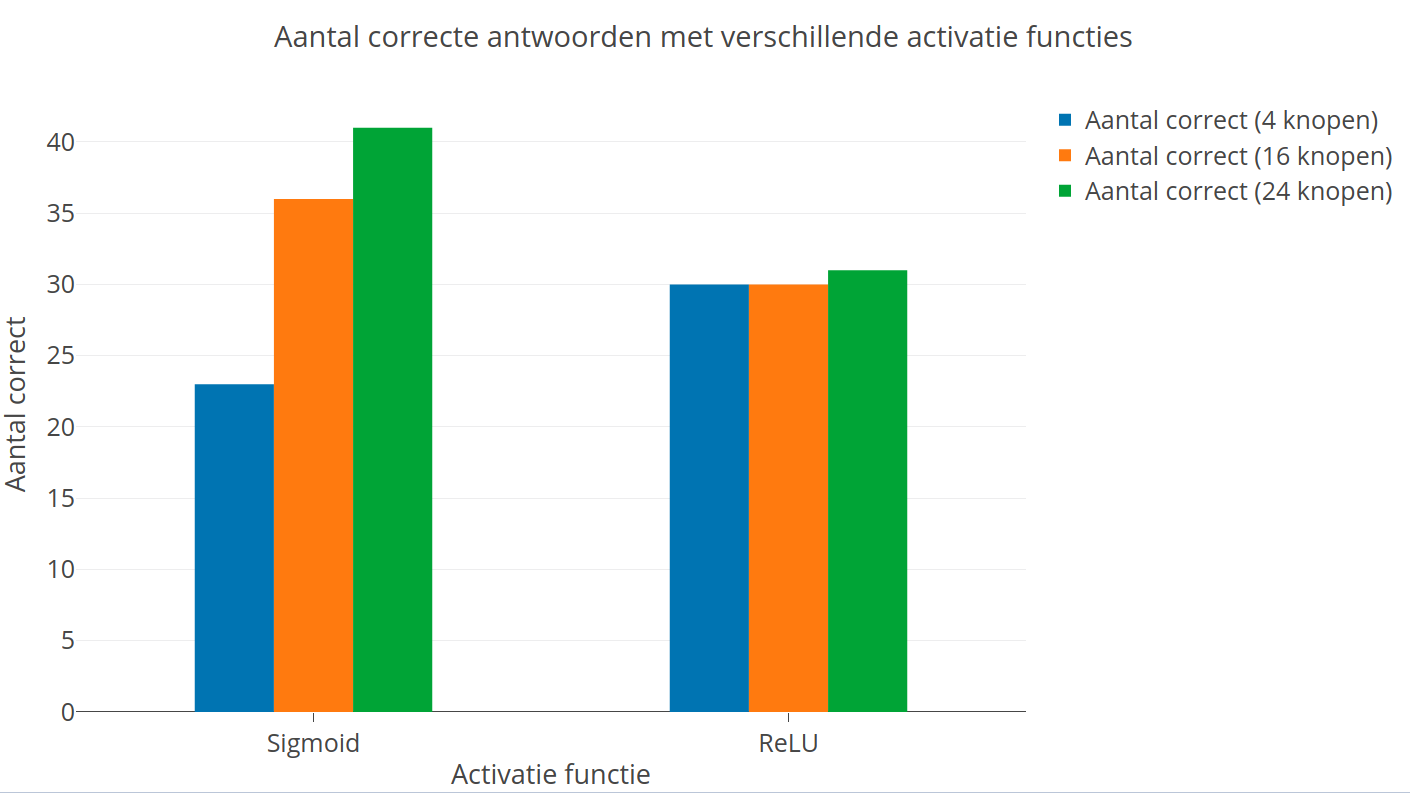
\includegraphics[scale=0.3]{graphs/g.png}
    \caption{Aantal correcte antwoorden over 50 executies met activatie functies sigmoid en ReLU met verschillende aantallen verborgen knopen}
    \label{fig:relu}
\end{figure}

\clearpage
\begin{figure}[ht!]
    \centering
    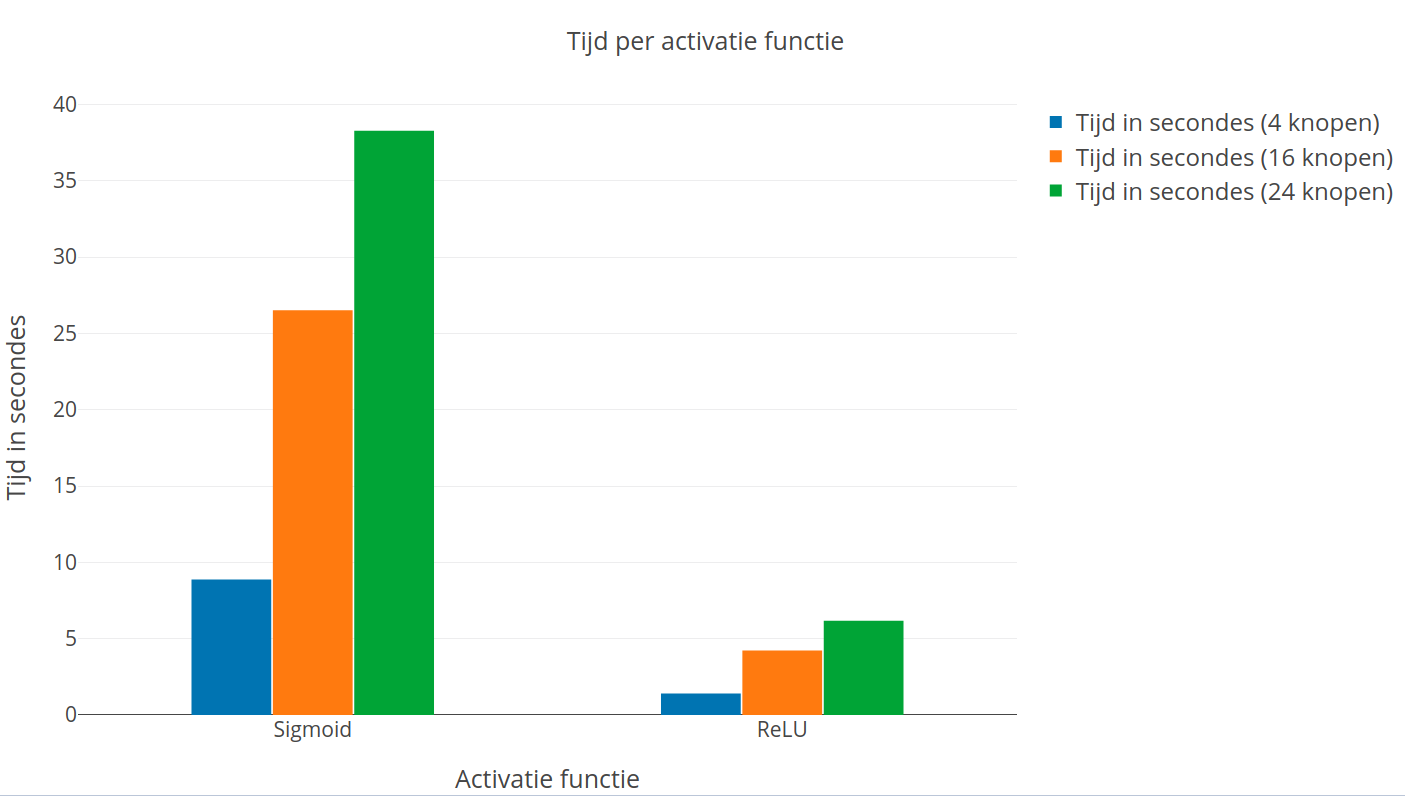
\includegraphics[scale=0.3]{graphs/time.png}
    \caption{Tijd in secondes over 50 executies met activatie functies sigmoid en ReLU met verschillende aantallen verborgen knopen}
    \label{fig:relutime}
\end{figure}

Tabel \ref{tab:relu} en Figuur \ref{fig:relu} laten het aantal correcte antwoorden van het netwerk zien met de activatie functies sigmoid en ReLU voor verschillend aantal verborgen knopen. We zien dat voor een klein aantal verborgen knopen, het netwerk beter leert met ReLU dan met sigmoid. Echter, bij grotere hoeveelheden knopen wordt dit omgedraaid en doet sigmoid het beter dan ReLU. Dit kan komen doordat ReLU geen bovengrens heeft en dus de output van het netwerk groter kan zijn dan 1. We zien wel dat ReLu significant sneller is dan sigmoid en dat de stijging veel sneller is bij sigmoid, zoals te zien op Figuur \ref{fig:relutime}.
Dit is een van de redenen waarom ReLU vaker wordt gebruikt in de praktijk, vooral bij diepere netwerken met meerdere verborgen lagen. Omdat het netwerk daar meer lagen heeft verwachten we dat ReLU beter presteert dan sigmoid in zowel tijd als correctheid. Dit kan worden onderzocht in een volgend onderzoek.